\subsection{Paired Escape from a Frozen Clot Envelope}
\label{sec:hull-escape-method}
For the transport benchmark we used three independently simulated 3D cylinders, each frozen at 0.01~s, 10~min and 30~min of mechanical evolution. In the native geometry, platelets were spheres of radius $1.13~\mu\mathrm m$; fibrin segments and cohesive links present in that frame were capsules of radius $0.05~\mu\mathrm m$. In the projected geometry, we clipped these solids to eight fixed $4~\mu\mathrm m$ sections, projected each section onto the $xy$ plane, and extended its footprint uniformly through that section. A tracer had to clear solids in neighboring sections as well as its own. This transformation changed the obstacles but not the mechanical snapshot.

For each pair, the common absorbing surface was the 3D convex hull of the native fibrin nodes (Fig.~\ref{fig:projection-geometry}A). This is an envelope that spans concavities, not a measured material interface. Projection changes the obstacles, not the dimensionality of the walk: the footprint blocks passage through the slab at that location, but a tracer can move around its side in $x$ or $y$ wherever there is clearance (Fig.~\ref{fig:projection-geometry}B,C).

\begin{figure*}[!t]
\centering
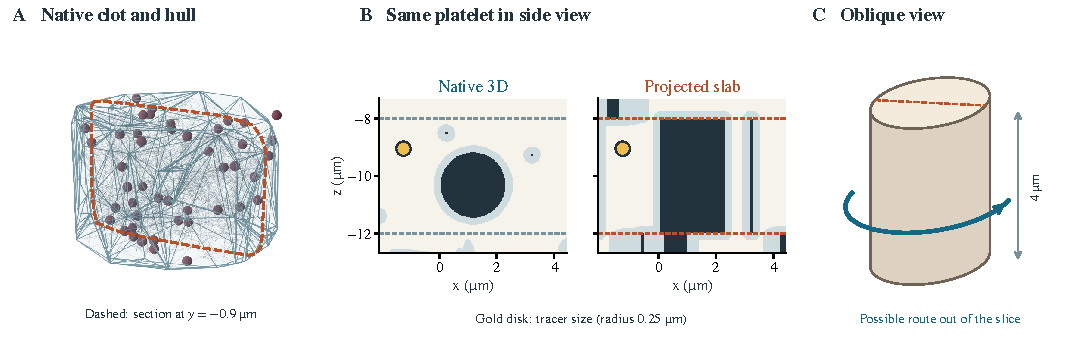
\includegraphics[width=\textwidth]{figures/seed1_projection_scheme.pdf}
\caption{What changes when a clot is projected? (A) Native simulated clot 1 at 0.01~s inside the absorbing hull of its fibrin nodes. (B) The same platelet in a fixed side slice: its native spherical profile leaves space above and below; its projected footprint extends from $z=-12$ to $-8~\mu\mathrm m$. Dark regions are solid; pale gray marks the additional clearance required for the tracer center. (C) Oblique view of this platelet's extruded footprint alone. The arrow illustrates a possible route around its side in three dimensions; it is not a recorded trajectory.}
\label{fig:projection-geometry}
\end{figure*}

We sampled 8,192 candidate tracer centers uniformly inside the hull and recorded which could accommodate a sphere of diameter $0.5~\mu\mathrm m$. For each valid position we searched for a path to any hull face using a six-neighbor grid spaced $1~\mu\mathrm m$ apart. Each path segment was checked against the continuous solids. A local search at $0.25~\mu\mathrm m$ spacing was used for unresolved positions. Finding a path certifies connectivity; failure to find one does not certify disconnection.

The admissible fraction counts \emph{center positions}: the center must be inside the hull and farther than one tracer radius from the physical solid. The hull itself is the absorbing surface for the center, so no extra clearance from it is required. Appendix~\ref{app:hull-fit} follows one frozen snapshot from the classification of candidate centers to escape from shared starts.

The first 768 randomly sampled positions valid in both geometries were used in the native clot, its projection and an empty copy of the same hull, irrespective of whether a route had been certified. We used matched Brownian increments with $D=0.4~\mu\mathrm m^2/\mathrm s$. At a solid contact the remaining increment was reflected about the local normal. Increments near the absorbing hull were subdivided using Brownian bridges. The primary base step was 0.025~s; 0.050 and 0.0125~s were also tested. No flow or binding was imposed.

Let $T$ be the first time the tracer center reaches the hull, and let $u$ denote elapsed transport time, distinct from the age of the frozen network. We measured survival and restricted mean survival time (RMST)~\cite{Redner2001,RoystonParmar2013}:
\begin{equation}
  S(u)=\Pr(T>u),\qquad
  \mathrm{RMST}_{\tau}=\int_0^\tau S(u)\,\mathrm du .
  \label{eq:hull-rmst}
\end{equation}
At $\tau=1{,}200$~s, RMST was estimated by averaging $\min(T,\tau)$, so a tracer still inside contributed the full observation time. Each clot received equal weight. For a relative delay, we first divided each clot's solid RMST by its empty-hull RMST, then averaged the ratios.

\subsection{Escape from Independently Generated Planar Stacks}
For each of the six $m=8$, $f_0=2.233$~nN stacks we froze the saved geometry at 0, 10 and 30~min. We extended its backbone segments, cohesive links present at that age, and platelet disks through their own $4~\mu\mathrm m$ slabs, with the same obstacle and tracer radii as above. The absorbing hull was built from fibrin nodes at their saved slab midplanes ($-14$ to $14~\mu\mathrm m$). To test this boundary choice, we also formed a hull from copies of the same node footprints at both faces of every slab ($-16$ to $16~\mu\mathrm m$), retaining the same obstacles. The primary hull used all three time steps; the alternative hull used the primary step.

For each stack, age and hull convention we sampled 8,192 uniform candidate centers. The first 768 admissible centers were used both in the stack and in its own empty hull, with matched Brownian increments and the same escape and connectivity rules as above. A start need not have a certified path. Starts were not matched between independently generated stacks and volumetric clots. The projected cohort's release sites were sampled uniformly in its admissible space: a position that fit after projecting and extruding the original solids also fit in the native clot. Thus projected and independent stacks use the same release \emph{rule}, not the same physical locations.
